\chapter{Inżynieria danych eksperymentalnych i testowe szablony modeli}
\section{Omówienie danych eksperymentalnych}

W celu zestawienia funkcjonalnego bibliotek uczenia maszynowego w języku C++ i przedstawienia przykładów konieczne było wybranie danych eksperymentalnych możliwych do wykorzystania jako porównawczy punkt odniesienia. W tym celu, dla pełnego przetestowania wybranych funkcjonalności przygotowano zestaw danych do problemu klasyfikacji binarnej oraz zadania regresji.

\subsection{Dane klasyfikacyjne}
	
	 Jako dane klasyfikacyjne wybrano bazę dotyczącą diagnostyki raka piersi ,,\textit{Wisconsin Diagnostic Breast Cancer}'' z listopada 1995 roku, w której zamieszczono wyniki obrazowania określone w sposób liczbowy. Autorami zestawu są Dr. Wiliam H. Wolberg, W. Nick Street oraz Olvi L. Mangasarian z Uniwersytetu Wisconsin \cite{wisconsin}. Baza ta jest dostępna do pobrania z repozytorium Uniwersytetu Californii \cite{Dua:2019}. Dane mają następującą strukturę:
	
	\begin{enumerate}
		\item [1)] ID - numer identyfikacyjny pacjentki;
		\item [2)] Diagnosis [\textit{Malignant - M} / \textit{Benign - B}] - charakter nowotworu, \textbf{zmienna odpowiedzi};
		\item [3)] Dane klasyfikujące:
			\begin{enumerate}
				\item [a)] \textit{Radius} - średnica guza;
				\item [b)] \textit{Texture} - tekstura guza;
				\item [c)] \textit{Perimeter} - obwód guza;
				\item [d)] \textit{Area} - pole guza;
				\item [e)] \textit{Smoothness} - gładkość, miara lokalnych różnic w promieniu guza;
				\item [f)] \textit{Compactness} - zwartość, wykorzystywana do oceny stadium guza;
				\item [g)] \textit{Concavity} - stopień wklęsłości miejsc guza;
				\item [h)] \textit{Concave points} - punkty wklęsłości guza;
				\item [i)] \textit{Symmetry} - symetria guza, pomagająca w ocenie charakteru przyrostu guza.
				\item [j)] \textit{Fractal dimention (,,coastline approximation'' - 1)} - wymiar fraktalny pozwalający na ilościowy opis złożoności komórek nerwowych, umożliwiający stwierdzenie nowotworzenia się zbioru komórek.
			\end{enumerate}
	\end{enumerate}
	
	Dla każdej ze zmiennych odpowiedzi została zebrana średnia wartość, odcyhelenie standardowe oraz średnia trzech największych pomiarów, gdzie każdy zestaw ustawiony jest sekwencyjnie (np. kolumna 3 - średni promień, kolumna 12 - odchylenie standardowe promienia, kolumna 22 - średnia trzech największych pomiarów promienia). Każda ze zmiennych ma charakter ciągły. Zredukowany zestaw danych, zawierający jedynie zmienne decyzyjne informujące o średnich wartościach znaleźć można jako dodatek do książki ,,\textit{Biostatistics Using JMP: A Practical Guide}'' autorstwa Trevora Bihla \cite{biostatisticsJMP}.
	
\subsection{Dane regresyjne}

	Do demonstracji problemu regresji wykorzystano zestaw danych ,,IronGlutathione'' dołączony do książki ,,Biostatistics Using JMP - A Practical Guide'' autorstwa Trevora Bihla \cite{biostatisticsJMP}, dotyczące badań nad związkiem między zawartością żelaza, a $\alpha$- i $\pi$-glutathonine-s-transferase w organiźmie człowieka. Obserwacje pochodzą z badań z 2012 roku. Zestaw posiada 90 obserwacji i składa się z 10 zmiennych:
	
	\begin{enumerate}
		\item \textit{Age} - wiek badanej osoby;
		\item \textit{Gender} - płeć osoby;
		\item \textit{Alpha GST (ng/L)} - zawartość transferazy glutatoninowej typu $\alpha$;
		\item \textit{pi GST (mg/L)} - zawartość transferazy glutatoninowej typi $\pi$;
		\item \textit{transferrin (mg/mL)} - zawartość transferyny;
		\item \textit{sTfR (mg/mL)} - zawartość rozpuszczalnego receptora transferyny;
		\item \textit{Iron (mg/dL)} - zawartość żelaza;
		\item \textit{TIBC (mg/dL)} - całkowita zdolność wiązania żelaza;
		\item \textit{\%ISAF (Iron / TIBC)} - współczynnik nasycenia transferyny;
		\item \textit{Ferritin (ng/dL)} - zawartość ferrytyny;
	\end{enumerate} 
	
	Z racji na większą swobode w wyborze zmiennej odpowiedzi w przypadku danych regresyjnych, zdecydowano się na wybór ostatniej zmiennej (\textit{Ferritin (ng/dL)}) jako przewidywaną zmienną odpowiedzi. 
	
\section{Charakterystyka i przetwarzenie danych}

	W celu przeprowadzenia procesu uczenia maszynowego, jednym z najistotniejszych kroków jakie należy podjąć jest wstępne zaznajomienie się z zestawem danych i jego analiza pod kątem rozkładu poszczególnych zmiennych oraz prawdopodobieństw. W tym celu wykorzystane zostało oprogramowanie JMP. 

	\subsection{Dane klasyfikacyjne}
	\subsubsection{Analiza rozkładu danych}
		
	Proces analizy rozkładu rozpoczęty został od przyjrzenia się zmiennej odpowiedzi (\textit{Diagnosis}). Rysunek \ref{fig:diagnosisdistribution} przedstawia uzyskany histogram, wraz z tabelą określającą ilość obserwacji danej klasy i współczynnik prawdopodobieństwa przynależności odpowiedzi do danej klasy. Zauważyć można, że dla użytego zestawu danych ilość zarejestrowano 357 obserwacji łagodnego raka piersi, a jego prawdopodobieństwo przynależności do klasy \textit{Benign} wynosi $\approx$ 62,7\%, natomiast do klasy \textit{Malignant} przynależało 212 obserwacji z prawodpodobieństwem $\approx$ 37,3\%.
		
	Podczas analizy histogramów zmiennych decyzyjnych, stwierdzono że znaczna ilość ma charakter prawostronnie skośny oraz występują dla nich obserwacje odstające, o czym informuje znajdujący się po prawej stronie histogramu wykres okienkowy (ang. \textit{box graph}), co przedstawiono na rysunku \ref{fig:variabledistribution}. Wyjątkiem okazała się zmienna \textit{Mean Largest Concave Points}), która mimo lekkiej skośności, okazała się nie posiadać obserwacji odstających. Na podstawie tych informacji stwierdzono, że aby przygotować dane w odpowiedni sposób do procesu uczenia należy przeprowadzić ich czyszczenie oraz normalizację rozkładu.
	
	\begin{figure}[!ht]
		\centering
		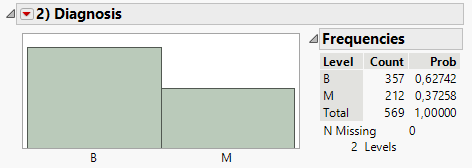
\includegraphics[width=0.6\linewidth]{Rysunki/Rozdzial2/diagnosis_distribution}
		\caption{Histogram rozkładu zmiennej odpowiedzi}
		\label{fig:diagnosisdistribution}
	\end{figure}
	
	\begin{figure}[!ht]
		\centering
		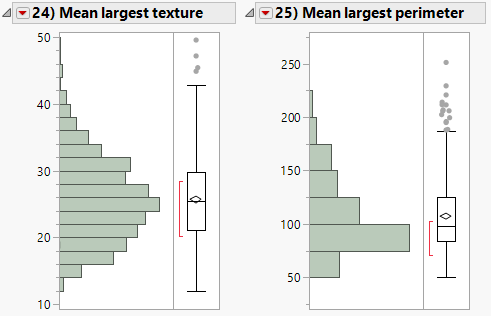
\includegraphics[width=0.6\linewidth]{Rysunki/Rozdzial2/variable_distribution}
		\caption{Przykłady histogramów zmiennych decyzyjnych}
		\label{fig:variabledistribution}
	\end{figure}
	
	
	\subsubsection{Czyszczenie i normalizacja rozkładu danych}
	
	Na pełny zestaw danych składa się 569 obserwacji. Podczas wstępnej analizy stwierdzono istnienie 13 brakujących wartości dla regresora \textit{Std err concave points}, dla których przyjęto wartość średnią z całej kolumny. Głównym problemem okazały się obserwacje odstające oraz skośności rozkładu. Do analizy obserwacji odstających wykorzystano wykresy okienkowe, gdzie oś Y reprezentowała zmienną odpowiedzi, natomiast oś X czyszczoną zmienną decyzyjną. Przykładowy wykres został przedstawiony na rysunku \ref{fig:boxgraph}. Ze względu na bardzo małą ilość obserwacji zdecydowano się rozpocząć proces przystosowywania danych do uczenia poprzez normalizację ich rozkładu, aby zminimalizować lub wyeliminować konieczność usunięcia danych odstających. 
	
	\begin{figure}[!ht]
		\centering
		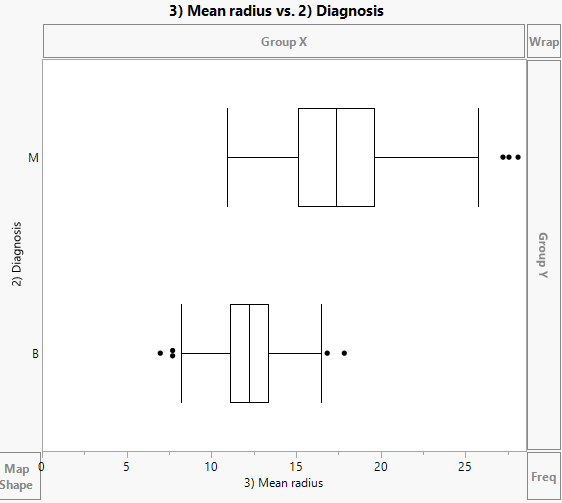
\includegraphics[width=0.7\linewidth]{Rysunki/Rozdzial2/box_graph}
		\caption{Przykład analizy obserwacji odstających dla poszczególnych klas zmiennej odpowiedzi}
		\label{fig:boxgraph}
	\end{figure}

	\newpage
	
	W pierwszym podejściu zdecydowano się na zastosowanie transformacji logarytmicznej dla wszystkich zmiennych decyzyjnych i porównanie charakterystyk uzyskanych rozkładów z oryginalnymi. Zmienna \textit{Mean largest concave points} okazała się posiadać rozkład bardzo zbliżony do standardowego, w związku z czym wyłączono ją z dalszej analizy normalizacji. Przykładowe wyniki przedstawiono na rysunku \ref{fig:log}. Transformacja ta okazała się skutecznym rozwiązaniem jedynie dla następujących zmiennych:
	
	\begin{enumerate}
		\item \textit{Mean radius};
		\item \textit{Mean texture};
		\item \textit{Mean perimeter},
		\item \textit{Mean area};
		\item \textit{Mean smoothness};
		\item \textit{Mean symmetry};
		\item \textit{Std err texture};
		\item \textit{Std err smoothness};
		\item \textit{Std err compactness};
		\item \textit{Std err concave points};
		\item \textit{Mean largest texture};
		\item \textit{Mean largest smoothness};
		\item \textit{Mean largest compactness}.
	\end{enumerate}

	\begin{figure}[!ht]
		\centering
		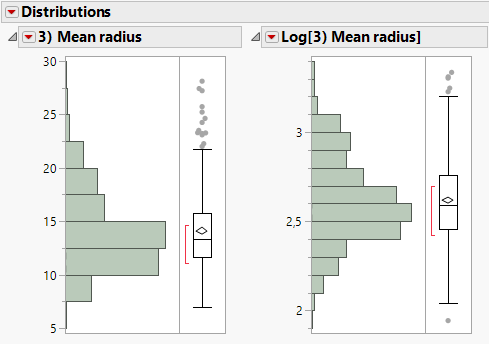
\includegraphics[width=0.7\linewidth]{Rysunki/Rozdzial3/log}
		\caption{Porównanie rozkładu danych przed i po transformacji logarytmicznej.}
		\label{fig:log}
	\end{figure}

	W drugim kroku podjęto próbę wykorzystania transformacji pierwiastkiem sześciennym dla pozostałych zmiennych decyzyjych, ze względu na jej skuteczność dla danych o rozkładzie prawoskośnym. Rysunek \ref{fig:cuberoot}. przedstawia porównanie rozkładu zmiennej \textit{Mean concavity} przed i po transfromacji pierwiastkiem sześciennym. Pomyślnie znormalizowano rozkład następujących zmiennych:
	
	\begin{enumerate}
		\item \textit{Mean compactness};
		\item \textit{Mean concavity};
		\item \textit{Mean concave points};
		\item \textit{Std err concavity};
		\item \textit{Mean largest radius};
		\item \textit{Mean largest perimeter};
		\item \textit{Mean largest concavity};
		\item \textit{Mean largest symmetry}.
	\end{enumerate} 

\begin{figure}[!ht]
	\centering
	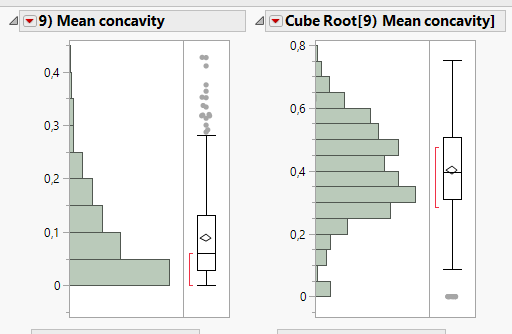
\includegraphics[width=0.7\linewidth]{Rysunki/Rozdzial3/cube_root}
	\caption{Porównanie rozkładów danych przed i po zastosowaniu transformacji pierwiastkiem sześciennym.}
	\label{fig:cuberoot}
\end{figure}

	Ostatecznym krokiem okazało się zastosownie odwrotnej transformacji Arrheniusa, Niestety część z uzyskanych zmodyfikowanych zmiennych decyzyjnych zachowała częściowy skośny rozkład, jednak inne przetestowane transformacje, jak m.in. pierwiastek kwadratowy, potęga kwadratowa, logarytm x+1, logarytm dziesiętny, funkcja potęgowa, funkcja wykładnicza, przyniosły rezultaty porównywalne lub gorsze od uzyskanego w wyniku w/w odwrotnej transformacji Arrheniusa. Rysunek \ref{fig:arrhenius} przedstawia porównanie uzyskanych rozkładów.
	
	\begin{figure}[!ht]
		\centering
		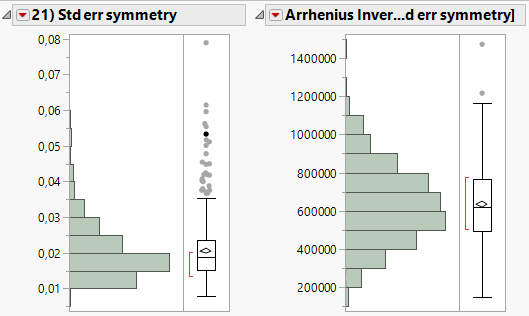
\includegraphics[width=0.7\linewidth]{Rysunki/Rozdzial3/arrhenius}
		\caption{Porównanie uzyskanych rozkładów danych przed i po odwrotnej transformacji Arrheniusa.}
		\label{fig:arrhenius}
	\end{figure}
	
	Ze względu na bardzo małą ilość obserwacji, zdecydowano się na zachowanie wszystkich obserwacji odstających, aby zapobiec utracie informacji i zmianie uzyskanych w procesie normalizacji rozkładów. W celu zachowania kompatybilności z bibliotekami omawianymi w niniejszej pracy, przekodowano zmienną odpowiedzi na wartości liczbowe.

	\subsection{Dane regresyjne}
	
	\subsubsection{Analiza rozkładu danych}
	
	Podobnie jak w przypadku danych klasyfikacyjnych, analizę rozpoczęto od zapoznania się z rozkładem wybranej zmiennej odpowiedzi. Zauważono że posiada ona rozkład skrajnie prawostronny, co przedstawiono na rysunku \ref{fig:ferritin}.
	
	\begin{figure}[!ht]
		\centering
		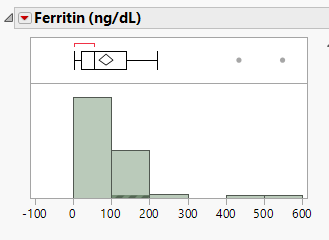
\includegraphics[width=0.5\linewidth]{Rozdzial3/ferritin}
		\caption{Wykres rozkładu zmiennej odpowiedzi dla zestawu regresyjnego}
		\label{fig:ferritin}
	\end{figure}
	
	Na wykresie okienkowym zawartym nad histogramem rozkładu zauważyć można wystąpienie dwóch obserwacji odstających. Podczas dalszej analizy, spostrzeżono podobny problem w przypadku zmiennych \textit{\%ISAF}, \textit{Iron}, \textit{sTfR}, \textit{Transferrin} oraz szczególnie \textit{Alpha GST}. Pozostałe zmienne charakteryzują się rozkładem zbliżonym do krzywej Gaussa, nie posiadając obserwacji zaklasyfikowanych jako odstające. Rysunek \ref{fig:decision} przedstawia dwa przykładowe histogramy rozkładów zmiennych decyzyjnych.
	
	\begin{figure}[!ht]
		\centering
		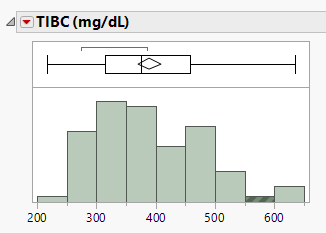
\includegraphics[width=0.6\linewidth]{Rozdzial3/decision}
		\caption{Przykłady rozkładu zmiennej decyzyjnej cz. 1}
		\label{fig:decision}
	\end{figure}

	\newpage
	\begin{figure}[!ht]
		\centering
		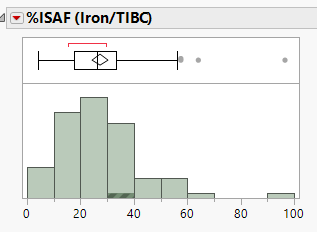
\includegraphics[width=0.6\linewidth]{Rozdzial3/decision1}
		\caption{Przykład rozkładu zmiennej decyzyjnej cz. 2}
		\label{fig:decision1}
	\end{figure}

	Pojedyncza zmienna - \textit{Gender} - posiada dychotomiczny charakter, aczkolwiek okazuje się relatywnie bardzo zrównoważona, posiadając rozkład na poziomie przynależności w 46,7\% do klasy F reprezentującej kobiety oraz 53,3\% do klasy M odpowiadającej mężczyznom. Rozkład tej zmiennej przedstawiono na rysunku \ref{fig:mnf}.
	
	\begin{figure}[!ht]
		\centering
		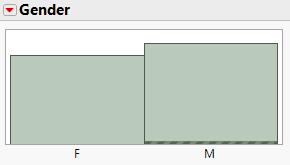
\includegraphics[width=0.6\linewidth]{Rozdzial3/mnf}
		\caption{Rozkład zmiennej Gender}
		\label{fig:mnf}
	\end{figure}
	
	\subsubsection{Czyszczenie i normalizacja rozkładu danych}
	
	W trakcie przeglądu obserwacji, zauważono pojedynczą obserwację z brakującą wartością zmiennej \textit{Ferritin}. Ze względu na wystąpienie tylko jednego takiego wpisu na 85 obserwacji, zdecydowano się na usunięcie jej. Pozostałymi kwestiami wymagającymi zaadresowania okazała się normalizacja rozkładu części zmiennych i decyzja o działaniu względem wartości odstających.
	
	W celu zmniejszenia ilości obserwacji odstających, postanowiono rozpocząć następny etap od problemu normalizacji rozkładu. Następujące zmienne, ze względu na ich obecną charakterystykę nie zostały poddane żadnym przekształceniom:
	
	\begin{enumerate}
		\item \textit{Age};
		\item \textit{Gender};
		\item \textit{TIBC}.
	\end{enumerate}

	Dla pozostałych zmiennych decyzyjnych zastosowano trzy rodzaje transformacji opisanych w sekcji omawiających dane klasyfikacyjne. Pierwszą z nich była obliczenie logarytmu z wartości zmiennej, które przyniosło zadowalający efekt dla zmiennych:
	
	\begin{enumerate}
		\item \textit{alpha GST};
		\item \textit{pi GST};
		\item \textit{sTfR};
		\item \textit{Ferritin} (zmienna odpowiedzi).
	\end{enumerate}

	Rysunek \ref{fig:log2} przedstawia przykład uzyskanej zmiany rozkładu dla zmiennej odpowiedzi.
	
	\begin{figure}[!ht]
		\centering
		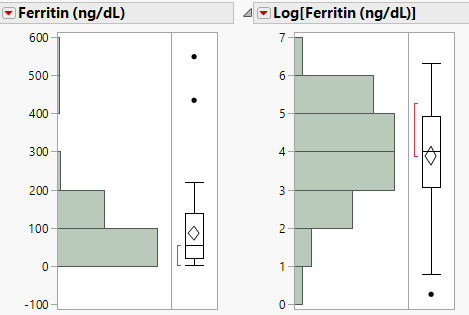
\includegraphics[width=0.7\linewidth]{Rozdzial3/log2}
		\caption{Wpływ transformacji logarytmicznej na rozkład zmiennej odpowiedzi}
		\label{fig:log2}
	\end{figure}

	Drugą transformacją o zadowalających wynikach okazało się zastosowanie pierwiastka kwadratowego, co pokazano na rysunku \ref{fig:cube2}. Wykorzystano ją do normalizacji rozkładu zmiennych:
	
	\begin{enumerate}
		\item \textit{Transferrin};
		\item \textit{Iron};
		\item \textit{\%ISAF}.
	\end{enumerate}

	\begin{figure}
		\centering
		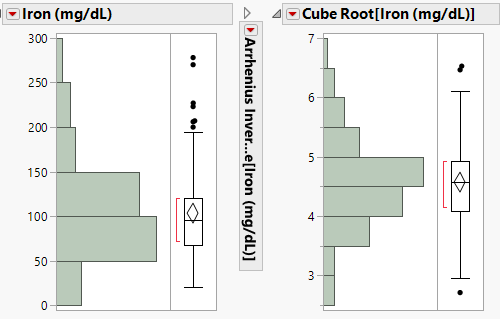
\includegraphics[width=0.7\linewidth]{Rozdzial3/cube2}
		\caption{Normalizacja rozkładu za pomocą transformacji pierwiastkiem kwadratowym.}
		\label{fig:cube2}
	\end{figure}

	Transformacja odwrotnym wzorem Arrheniusa okazała się nieskuteczna na wszystkich zmiennych, uzyskując gorsze efekty niż pozostałe przedstawione wyżej metody. Z racji na niewielką ilość obserwacji, oraz stosunkowo małą liczbę wartości odstających, zdecydowano się na pozostawienie ich do procesu uczenia. W celu kompatybilności z omawianymi bibliotekami, przekodowano zmienną dychotomiczną na wartości liczbowe.

\section{Szablony docelowych modeli dla zadanych danych eksperymentalnych}

W trakcie analizy zestawów danych wybrany został przedstawiony poniżej zestaw metod dla których wykonano i podsumowano testy praktyczne. Szablony struktury rozwiązań, takie jak np. wybór zmiennych uczestniczących w procesie uczenia, lub struktura sieci neuronowej zostały ustalone w sposób empiryczny z wykorzystaniem programu do uczenia maszynowego JMP. 

%\subsection{Regresja logistyczna}

%Badanie zależności w modelu regresji logistycznej odbyło się z wykorzystaniem wykresu wpływu zmiennej decyzyjnej na zmienną odpowiedzi opartego o p-wartość. Jako próg pozwalający na odrzucenie hipotezy zerowej (hipotezy o braku wypływu zmiennej na odpowiedź) przyjęto 0,05 jednostek. Rysunek \ref{fig:pvalue1} przedstawia w/w wykres wraz z p-wartościami dla poszczególnych zmiennych. Zauważyć można, że dla części zmiennych nie została wyznaczona p-wartość -- oznacza to, że część zmiennych jest ze sobą skorelowanych.

%Pierwszym krokiem w wybraniu istotnych zmiennych było usunięcie zmiennych skorelowanych, drugim natomiast stopniowe usuwanie zmiennych o p-wartości powyżej określonego progu. Rysunek \ref{fig:pvalue2} przedstawia listę wraz z wykresem kolumnowym istotnych regresorów. Ich lista, wraz z odpowiadającymi im p-wartościami została umieszczona w tabeli \ref{lin_reg:1}.

%\begin{table}
%	\centering
%	\begin{tabular}{l|c}
%		Nazwa zmiennej & p-wartość \\
%		\hline
%		\textit{Log mean largest texture} & 0,00000 \\
%		\textit{Log mean largest compactness} & 0,00000 \\
%		\textit{Cube root mean largest symmetry} & 0,00001 \\
%		\textit{Arrhenius inverse std err symmetry} & 0,00005 \\
%		\textit{Arrhenius inverse std err radius} & 0,00018 \\
%		\textit{Cube root mean concave points} & 0,00056 \\
%		\textit{Cube root mean largest concavity} & 0,00069 \\
%		\textit{Log std err texture} & 0,00252 \\
%		\textit{Cube root mean largest perimeter} & 0,00526 \\
%		\textit{Log mean smoothness} & 0,04867 \\
%		\textit{Log mean radius} & 0,04884
%	\end{tabular}
%	\caption{Lista istotnych regresorów}
%	\label{lin_reg:1}
%\end{table}

%\begin{figure}[!ht]
%	\centering
%	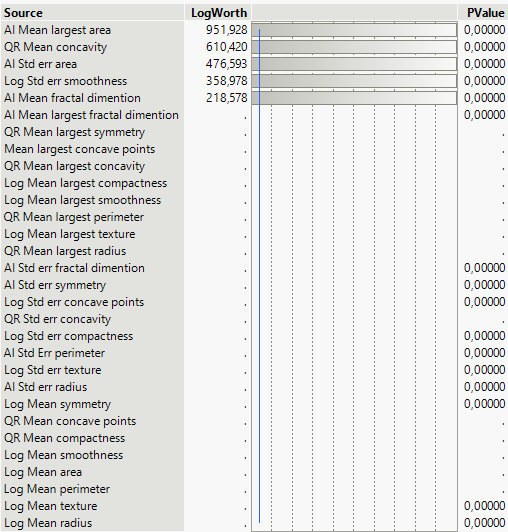
\includegraphics[width=0.9\linewidth]{Rysunki/Rozdzial3/pvalue1}
%	\caption{Wykres p-wartości dla całego zestawu zmiennych decyzyjnych.}
%	\label{fig:pvalue1}
%\end{figure}

%\newpage
%Dla wybranego zestawu zmiennych model osiągnął dokładność na poziomie $R^{2}$ = 0.9401. Zgodnie z macierzą pomyłek, 207 obserwacji typu \textit{Malignant} oraz 335 obserwacji \textit{Benign} zostało zaklasyfikowanych poprawnie. Oznacza to, że model uzyskał tylko 2 wyniki typu \textit{false-positive} (prawdopodobieństwo 0,6\%) i 5 wyników typu \textit{false-negative} (prawdopodobieństwo 2,4\%) dla danych treningowych. Ze względu na mały zestaw obserwacji, ryzyko przeuczenia jest znikome, w związku z czym nie wytypowano zestawu danych walidacyjnych. Rysunek \ref{fig:roc} przedstawia krzywą charakterystyczną odbiornika dla modelu. 

%\begin{figure}[!ht]
%	\centering
%	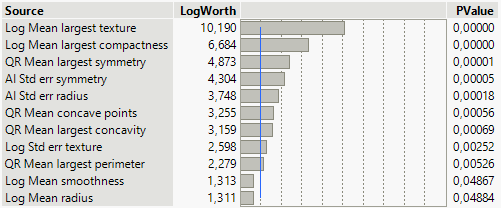
\includegraphics[width=0.7\linewidth]{Rysunki/Rozdzial3/pvalue2}
%	\caption{Wykres i p-wartości istotnych zmiennych decyzyjnych}
%	\label{fig:pvalue2}
%\end{figure}

%\begin{figure}[!ht]
%	\centering
%	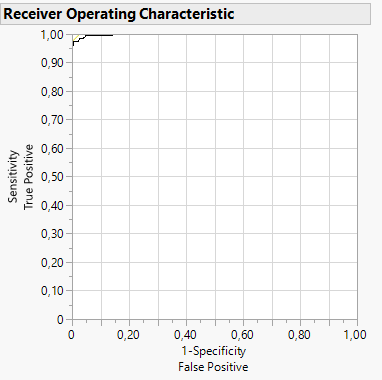
\includegraphics[width=0.5\linewidth]{Rysunki/Rozdzial3/roc}
%	\caption{Krzywa charakterystyczna odbiornika (ROC) dla modelu regresji logistycznej}
%	\label{fig:roc}
%\end{figure}

%\subsection{Głęboka sieć neuronowa}

%Do przygotowania sieci neuronowej wykorzystano zestaw zmiennych zawartych w tabeli \ref{lin_reg:1}. Dane zostały losowo podzielony na dane uczące i walidacyjne w propocji 80\% do 20\%. W wyniku prób i błędów, optymalny model uzyskano przy strukturze przedstawionej w tabeli \ref{neural:1}. Graficzny schemat struktury został także przedstawiony na rysunku \ref{fig:neuralstruct}.

%\begin{table}[!ht]
%	\centering
%	\begin{tabular}{c|c|c}
%		Typ warstwy & ilość neuronów & aktywacja \\
%		\hline
%		ukryta & 5 & tangens hiperboliczny \\
%		ukryta & 5 & tangens hiperboliczny \\
%		wyjściowa & 2 & ---	
%	\end{tabular}
%	\caption{Struktura modelu sieci neuronowej}
%	\label{neural:1}
%\end{table}

%\begin{figure}[!ht]
%	\centering
%	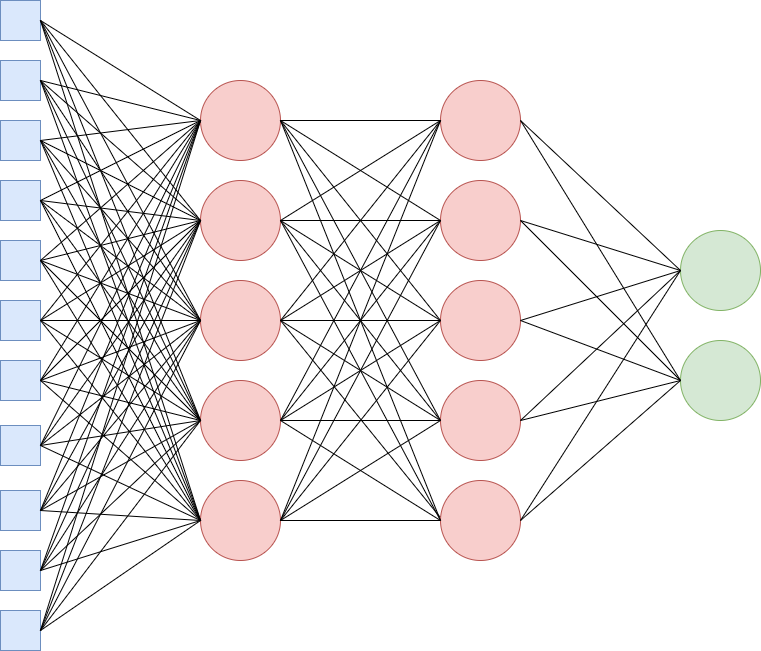
\includegraphics[width=0.6\linewidth]{Rysunki/Rozdzial3/neural_struct}
%	\caption{Schemat struktury sieci}
%	\label{fig:neuralstruct}
%\end{figure}

%Środowisko JMP nie udostępnia informacji o funkcji aktywacji warstwy wyjściowej, w związku z czym w tabeli 3.2 została ona pominięta. Dla ziarna o wartości 1234 uzyskano model którego statystyka $R^{2}$ dla danych treningowych wyniosła 0.966268, natomiast dla danych testowych 0.9924547. Trafność dla losowo wybranego zestawu testowego wyniosła 100\%, natomiast dla danych uczących napotkano 5 przypadków \textit{false-negative} (prawdopodobieństwo 3\%) oraz 1 przypadek \textit{false-positive} (prawdopodobieństwo 0,4\%). Rysunki \ref{fig:roctest} oraz \ref{fig:rocvalid} przedstawiają krzywe charakterystyczne odbiornika dla zestawu testowego i walidacyjnego.

%\begin{figure}[!ht]
%	\begin{minipage}{0.48\textwidth}
%			\centering
%			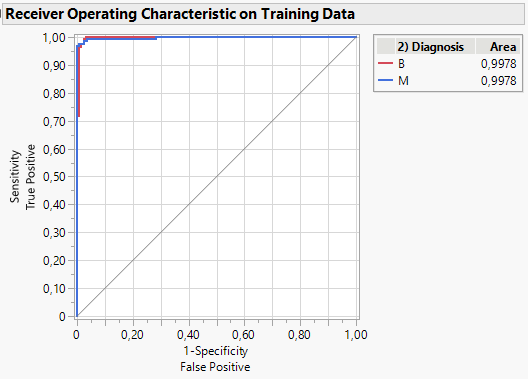
\includegraphics[width=0.95\linewidth]{Rysunki/Rozdzial3/roc_test}
%			\caption{Krzywa charakterysty-czna odbiornika dla zestawu testowego}
%			\label{fig:roctest}
%	\end{minipage}%
%	\hspace{8pt}
%	\begin{minipage}{0.48\textwidth}
%			\centering
%			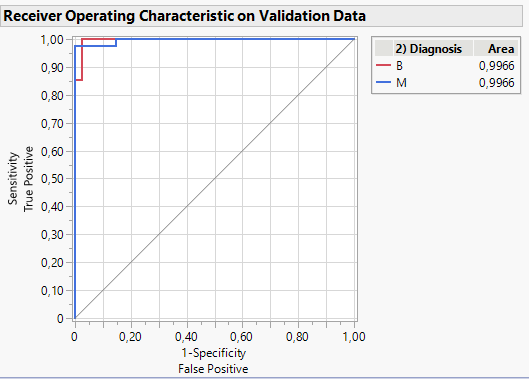
\includegraphics[width=0.95\linewidth]{Rysunki/Rozdzial3/roc_valid}
%			\caption{Krzywa charakterysty-czna odbiornika dla danych walidacyjnych}
%			\label{fig:rocvalid}
%	\end{minipage}
%\end{figure}

\subsection{Maszyna wektorów nośnych}

Do predykcji diagnozy wykorzystano ten sam zestaw regresorów, zawartych w tabeli 3.1. Ponownie w celu walidacji użyto metody wybrania losowego zestawu walidacyjnego spośród dostarczonych danych, w proporcji 80\% obserwacji uczących i 20\% testowych, z użyciem wartości 1234 dla ziarna generatora liczb pseudolosowych. Jako funkcję jądra maszyny wektorów nośnych (ang. Support Vector Machine, SVM) wybrano \textit{Radial Basis Function}, która jest domyślnym wyborem dla SVM w środowisku JMP. 

\begin{longtable}{l | c}
	\centering
	Zmienna decyzyjna & wartość X \\
	\hline
	\textit{Log mean largest texture} & 3,217 \\
	\textit{Log mean largest compactness} & -1,5504 \\
	\textit{Cube root mean largest symmetry} & 0,65891 \\
	\textit{Arrhenius inverse std err symmetry} & 635100 \\
	\textit{Arrhenius inverse std err radius} & 38170 \\
	\textit{Cube root mean concave points} & 0,33665 \\
	\textit{Cube root mean largest concavity} & 0,5951 \\
	\textit{Log std err texture} & 0,1049 \\
	\textit{Cube root mean largest perimeter} & 4,7045 \\
	\textit{Log mean smoothness} & -2,3502 \\
	\textit{Log mean radius} & 2,6191 \\
	\caption{Wartości składowych X modelu dla poszczególnych zmiennych decyzyjnych}
	\label{svm:1}
\end{longtable} 

\begin{figure}[!ht]
	\begin{minipage}{0.48\textwidth}
		\centering
		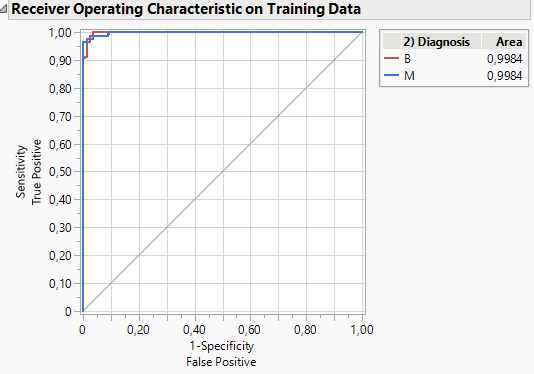
\includegraphics[width=0.98\linewidth]{Rysunki/Rozdzial3/roc_svm1_test}
		\caption{Krzywa charakterystycz-na odbiornika dla danych uczących modelu SVM}
		\label{fig:rocsvm1test}		
	\end{minipage}%
	\hspace{10pt}
	\begin{minipage}{0.48\textwidth}
		\centering
		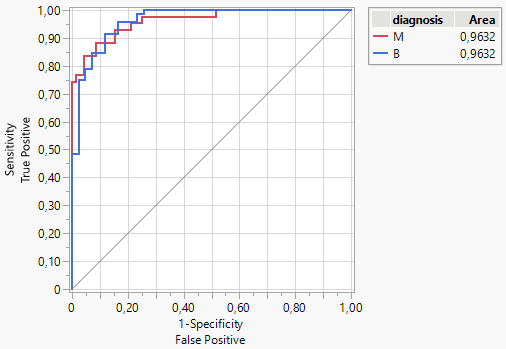
\includegraphics[width=0.98\linewidth]{Rysunki/Rozdzial3/roc_svm1_val}
		\caption{Krzywa charakterystycz-na odbiornika dla danych walidacyjnych modelu SVM}
		\label{fig:rocsvm1val}				
	\end{minipage}	
\end{figure}

Utworzony w ten sposób model posiada generalizowaną statystykę $R^{2}$ na poziomie 0.97161 dla zestawu walidacyjnego, i uzyskał wskaźnik błędnej klasyfikacji wynoszący 0\% dla danych testowych, oraz 1,3\% dla danych uczących. Tabela \ref{svm:1} przedstawia wartości X dla poszczególnych regresorów. Rysunki \ref{fig:rocsvm1test} oraz \ref{fig:rocsvm1val} przedstawiają krzywe charakterystyczne odbiornika dla uzyskanego modelu, pola pod którymi uzyskały wartość odpowiednio 0,9984 dla danych uczących i 1 dla danych testowych.

\subsection{Regresja liniowa}

Podobnie jak w przypadku regresji logistycznej, do ustalenia które z regresorów mają największy wpływ na zmienną odpowiedzi zastosowano wykres wpływu poszczególnych zmiennych oparty o p-wartość. Jako próg zaakceptowania parametru do procesu uczenia zdecydowano się na wybranie p-wartości wynoszących poniżej 0,05 jednostek. Rysunek \ref{fig:pvalue3} przedstawia wykres dla wszystkich zmiennych, natomiast rysunek \ref{fig:pvalue4} ukazuje wykres zawierający jedynie wybrane zmienne. 

\begin{figure}[!ht]
	\centering
	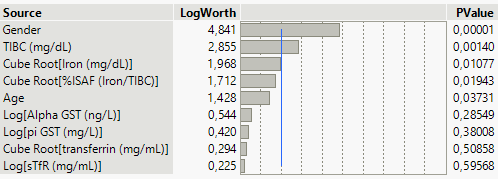
\includegraphics[width=\linewidth]{Rozdzial3/pvalue3}
	\caption{Wykres p-wartości dla wszystkich zmiennych}
	\label{fig:pvalue3}
\end{figure}

\begin{figure}[!ht]
	\centering
	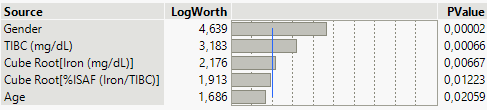
\includegraphics[width=\linewidth]{Rozdzial3/pvalue4}
	\caption{Wykres p-wartości dla zmiennych wybranych do procesu uczenia}
	\label{fig:pvalue4}
\end{figure}

W procesie eliminacji regresorów o p-wartości przekraczającej wybrany próg akceptacji, wybrano następujące zmienne do procesu uczenia:

\begin{table}[!ht]
	\begin{minipage}{0.48\textwidth}
		\centering
		\begin{tabular}{l|c}
			Nazwa zmiennej & p-wartość \\
			\hline
			\textit{Gender} & 0.00002 \\
			\textit{TIBC} & 0.00066 \\
			\textit{Cube Root Iron} & 0.00667 \\
			\textit{Cube Root \%ISAF} & 0.01223 \\
			\textit{Age} & 0.02059
		\end{tabular}
		\caption{Wybrane zmienne decyzyjne i ich p-wartości}
		\label{pvalue}
	\end{minipage}%
	\hspace{0.04\textwidth}
	\begin{minipage}{0.48\textwidth}
		\centering
		\begin{tabular}{l|c}
			Nazwa zmiennej & waga \\
			\hline
			\textit{Intercept} & 8,498959 \\
			\textit{Age} & 0.0201022 \\
			\textit{Gender[F - M]} & -0.959795 \\
			\textit{Cube Root Iron} & 2,9461861 \\
			\textit{TIBC} & -0.014182 \\
			\textit{Cube Root \%ISAF} & -4,356345
		\end{tabular}
		\caption{wartości wag zmiennych decyzyjnych}
		\label{weights}		
	\end{minipage}
\end{table}

W wyniku uczenia uzyskano model którego wartość metryki \textit{$R^2$} wyniosła 0.4654525, co sugeruje że dane są słabo aproksymowalne liniowo. Tabela \ref{weights} przedstawia nauczone wagi poszczególnych regresorów.